\chapter{Heat and Phases of Matter}

Put a cold metal spoon in hot cocoa, and the spoon warms while the cocoa cools. Leave ice in a glass, and
it melts without getting any warmer than 0\textdegree C. A rice cooker somehow knows exactly when the rice is
done. In the Temperature and the Gas Laws chapter, you saw that temperature is the motion of molecules. This
chapter follows that energy as it flows from hot things to cold things, and as it melts, boils, and freezes
matter.

\section{Heat}\label{chap:heat}\index{heat}
All mass in the universe has heat, whether you are looking at a block of dry ice (frozen $CO_2$, $-78.5^\circ$ C)
or the surface of the sun ($5,600^\circ$ C). As long as the mass is above absolute zero --- the \index{absolute zero}coldest possible
temperature in the universe --- there is some amount of heat in it.

\subsection{How Heat Works}

As you heat up an object, you are imparting energy into it. Where does this energy go? The atoms take this energy
and they begin to move, vibrating and bumping into each other, causing the heat to spread throughout. Every time the
atoms collide and bounce off of each other, they emit a tiny amount of energy as light. In most cases, that light is
in the \index{infrared}infrared spectrum, but in extreme cases can be visible, such as with molten lava or hot metal.

As objects interact, they either put heat into colder objects or take heat from warmer objects. That is what allows you to heat up
anything in the first place. The hot air from a stove or bunsen burner interacts with the pan or test tube you are heating,
passing the air's heat on. How could you model this?

\subsection{Specific Heat Capacity}

If you are heating something, the amount of energy you need to
transfer to it depends on three things: the mass of the thing you are
heating, the amount of temperature change you want, and the
\textit{specific heat capacity} of that substance.\index{specific heat capacity}

\begin{mdframed}[style=important, frametitle={Energy in Heat Transfer}]

  The energy moved in a heat transfer is given by

  $$E = m c \Delta T$$

  \index{heat transfer}

  where $m$ is the mass, $\Delta T$ is the change in temperature, and
  $c$ is the specific heat capacity of the substance.
% ADD: q=mcat

  (Note that this
  assumes there is not a \index{phase change}phase change. For example, this formula works nicely on
  warming liquid water, but it gets more complicated if you warm the
  water past its boiling point.)

\end{mdframed}

Can we guess the specific heat capacity of a substance? It is very,
very difficult to guess the specific heat of a substance, so we determine
it by experimentation.

For example, it takes 0.9 joules to raise
the temperature of solid aluminum one degree Celsius. So we say ``The
specific heat capacity of aluminum is 0.9 J/g $^\circ$C.''

The specific heat capacity of liquid water is about 4.2 J/g $^\circ$C.

Let us say you put a 1 kg aluminum pan that is $80^\circ$ C into
3 liters of water that is $20^\circ$ C. Energy, in the form of heat,
will be transferred from the pan to the water until they are at the same
temperature. We call this ``thermal equilibrium''.\index{thermal equilibrium}

What will the temperature of the water be?

To answer this question, the amount of energy given off by the
pan must equal the amount of energy absorbed by the water. They also
need to be the same temperature at the end. Let $T$ be the final
temperature of both.

3 liters of water weighs 3,000 grams, so the
change in energy in the water will be:

$$E_W = m c \Delta_T = (3000)(4.2)(T - 20) = 12600T - 252000 \text{ joules}$$

The pan weighs 1000 grams, so the change in energy in the pan will be::

$$E_P = m c \Delta_T = (1000)(0.9)(T - 80) = 900T - 72000 \text{ joules}$$

The total energy stays the same, so $E_W + E_P = 0$. This means you need to solve

$$(12600T - 252000) + (900T - 72000) = 0$$

And find that the temperature at equilibrium will be

$$T = 24^\circ \text{C}$$

\begin{Exercise}[title={Thermal Equilibrium}, label=thermal_equilibrium]

Just as you put the aluminium pan in the water as described above,
someone also puts a 1.2 kg block of copper cooled to 10 $^\circ$ C.
The specific heat of solid copper is about 0.4 J/g $^\circ$C.

What is the new temperature at equilibrium?

\end{Exercise}
\begin{Answer}[ref=thermal_equilibrium]

  $$E_C = (1200)(0.4)(T - 10) = 480T - 4800$$

Total energy stays constant:

$$0 = (12600T - 252000) + (900T - 72000) + (480T - 4800)$$

Solving for $T$ gets you $T = 23.52^\circ$ C.

\end{Answer}

\subsection{Getting to Equilibrium}

When two objects with different temperatures are touching, the speed
at which they exchange heat is proportional to the differences in
their temperatures. As their temperatures get closer together,
the heat exchange slows down.
% ADD: explain which object, water or metal has a greater temperature change

In our example, the pan and the water will get close to equilibrium
quickly, but they may never actually reach equilibrium.

\begin{tikzpicture}
    \begin{axis}[
        xmin=0,xmax=4.25,
        ymin=15,ymax=85,
        axis x line=middle,
        axis y line=middle,
        axis line style=<->,
        xlabel={minutes},
        ylabel={degrees celsius},
        ]
        \addplot[no marks,sdkblue] expression[domain=0:4,samples=100]{24 + 56 * pow(2,-1.5 * x)} node[above, xshift=-1cm, yshift=0.1cm]{Pan};
        \addplot[no marks,sdkblue] expression[domain=0:4,samples=100]{24 - 4 * pow(2,-0.8 * x)} node[below, xshift=-2.5cm]{Water};
        \addplot[no marks,dashed,gray] coordinates {(0,24)(6,24)} node[above, xshift=-8cm]{equilibrium};
    \end{axis}
\end{tikzpicture}

\begin{Exercise}[title={Cooling Your Coffee}, label=cool_coffee]

  You have been given a ridiculously hot cup of coffee and a small pitcher of chilled milk.

  You need to start chugging your coffee in three minutes, and you want it as cool as possible at that time. When should you add the milk to the coffee?

\end{Exercise}
\begin{Answer}[ref=cool_coffee]

  During the 3 minutes, you want the coffee to give off as much of its
  heat as possible, so you want to maximize the difference between the
  temperature of the coffee and the temperature of the room around
  it.

  You wait until the last moment to put the milk in.

\end{Answer}

\subsection{Specific Heat Capacity Details}

For any given substance, the specific heat capacity often changes a
great deal when the substance changes state. For example, ice is 2.1 J/g
$^\circ$C, whereas liquid water is 4.2 J/g$^\circ$C.

Even within a given state, the specific heat capacity varies a bit
based on the temperature and pressure. If you are trying to do these
sorts of calculations with great accuracy, you will want to find the
specific heat capacity that matches your situation. For example, you
might look for the specific heat capacity for water at $22^\circ$C at
1 atmosphere of pressure (atm).


\section{Phases of Matter}
You have experienced $H_2O$ in three phases of matter:
\begin{itemize}
\item Ice is $H_2O$ in the solid phase. At standard pressure, when the temperature of $H_2O$ is below $0^\circ$ C, it is a solid. 
\item Water is $H_2O$ in the liquid phase. At standard pressure, when the temperature of $H_2O$ is between $0^\circ$ C and $100^\circ$ C, it is a liquid.
\item Water vapor (or steam) is the gas phase. At standard pressure, when the temperature of $H_2O$ is above $100^\circ$ C, it is a gas.
\end{itemize}

Let us look at some of the properties of the three phases:

\begin{tabular}{p{5cm}|p{5cm}|p{5cm}}
Gas & Liquid & Solid \\
\hline
Assumes the volume and shape of its container & 
Assumes the shape, but not the volume, of its container &
Retains its shape and volume \\
\hline
Compressible & Not compressible & Not compressible \\
\end{tabular}

\subsection{Thinking Microscopically About Phase}

As mentioned earlier in this chapter, there are intermolecular forces that attract molecules to each
other. A pair of molecules will have very strong intermolecular forces or very weak intermolecular forces,
depending on what atoms they are made of.

For example, two helium atoms are only very weakly attracted to each other. The particles in $NaCl$ (table salt), on the other hand, attract each other very strongly.

In a gas, the molecules have lots of room to roam and lots of kinetic energy: The intermolecular attraction has very little effect.

In a liquid, the molecules are sticking close together, but are still moving around, sort of like bees in a hive.

In a solid, the molecules are not changing their configuration, and the kinetic energy they have is just expressed as vibrations within that configuration. You can imagine them like eggs vibrating in a carton.

As you would expect, molecules with strong intermolecular attraction require more kinetic energy to change phases. For example, helium is a liquid below $-269^\circ$ C. $NaCl$, on the other hand, is a liquid between $801^\circ$ and $1,413^\circ$ C. 

These temperatures are at standard pressure (100 kPa or 1 atm). Pressure also has a role in phase change. In low pressure environments, it is much easier for the molecules to make the jump to being a gas.

For example, if you climb a mountain until the atmospheric pressure is 70 kPa, your water will boil at about $90^\circ$ C. 

If you rise in a balloon until the atmospheric pressure is 500 Pa, water cannot be liquid at any temperature. Ice turns directly into vapor, and liquid water never appears. There is no liquid water at 500 Pa!

For any molecule, we could observe its phase at a wide range of temperatures and pressures. This would let us create a phase diagram. \index{phase diagram}Here is the phase diagram for $H_2O$:

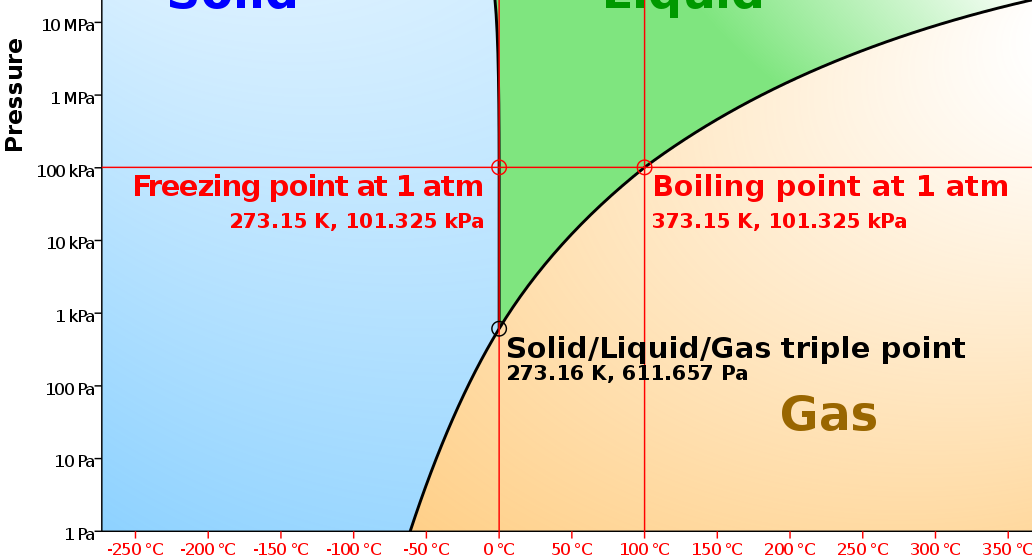
\includegraphics[width=\textwidth]{waterphase_edit.png}


\subsection{Phase Changes and Energy}\index{phase change}

The molar heat capacity of ice is about 37.7 J/mol-K. That is, it takes about 37.7 Joules of energy to raise the temperature of one mole of ice by one degree kelvin.

The molar heat capacity of liquid water is about 75.4 J/mol-K. For water vapor, it is about 36.6 J/mol-K.

Imagine you have mole of ice at 173 K, and you are going to gradually add kinetic energy into it until you have steam at 473 K. You might guess (incorrectly) that the temperature vs. energy applied would look like this:
\begin{figure}[H]
    \centering
    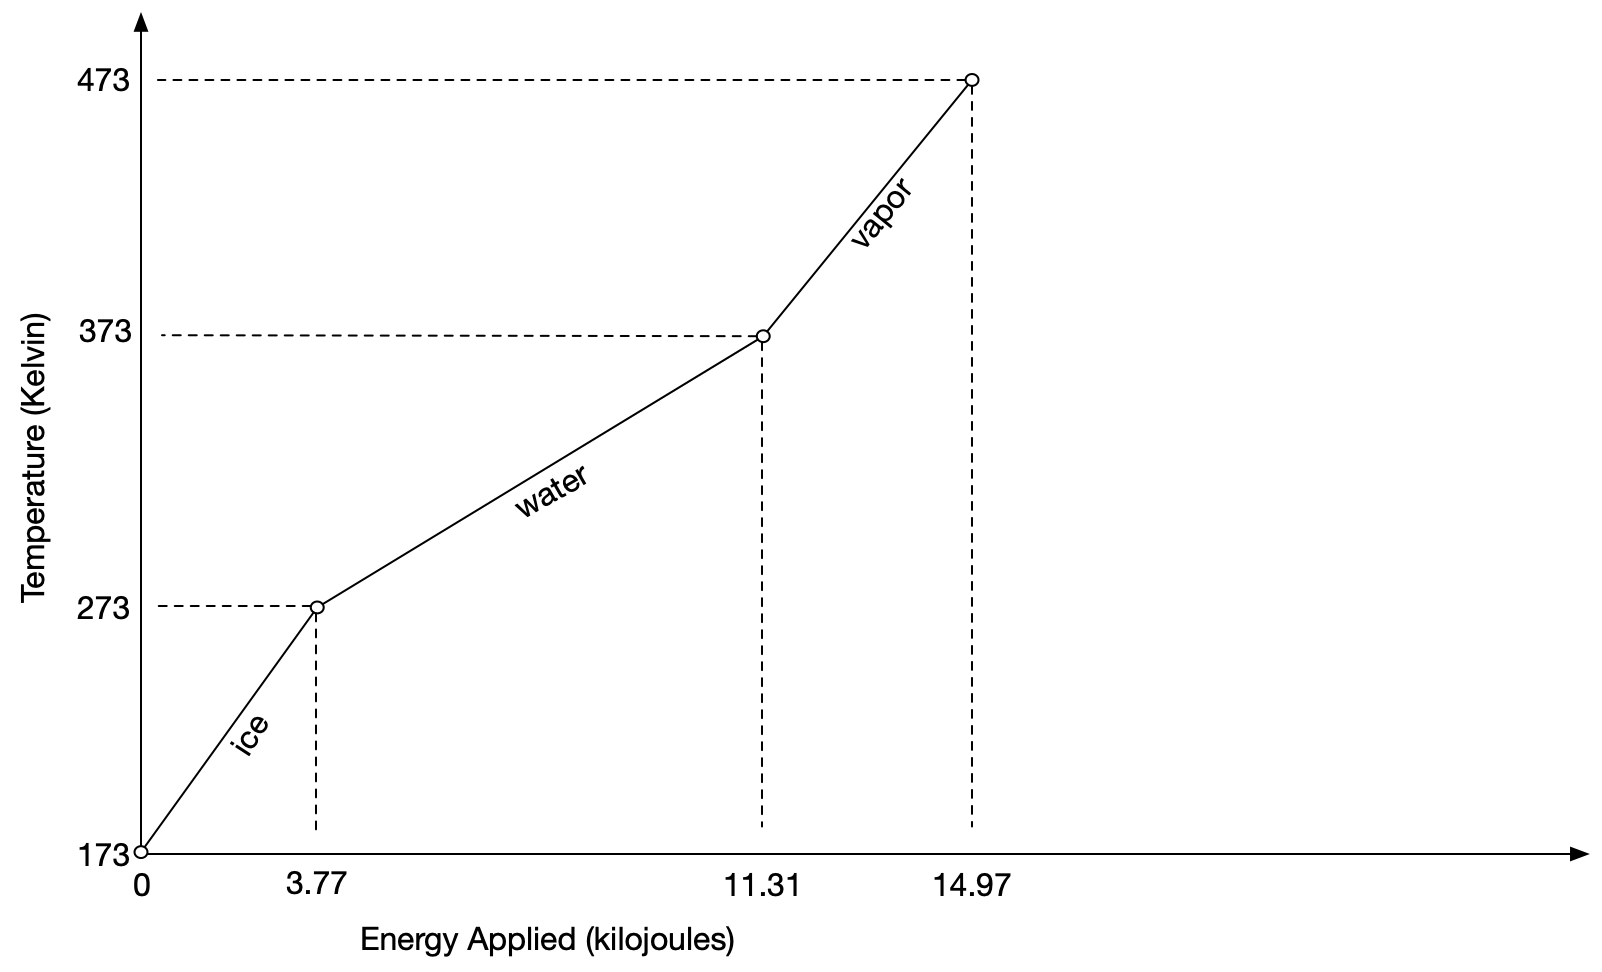
\includegraphics[width=0.8\linewidth]{energynaive.png}
    \caption{Assumption of temperature vs. energy applied.}
    \label{fig:energy1}
\end{figure}

However, once molecules are nestled into their solid state (like eggs in cartons), it takes extra energy to make them move like a liquid. How much more energy? For water, it is 6.01 kilojoules per mole. This is known as \newterm{the latent heat of melting} or \index{heat of fusion}\newterm{the heat of fusion}.

Similarly, the transition from liquid to gas takes energy. At standard pressure, converting a mole of liquid water to vapor requires $40.7$ kilojoules per mole. This is known as \index{latent heat!vaporization}\newterm{the latent heat of vaporization}. So, the graph would actually look like this:
\begin{figure}[H]
    \centering
    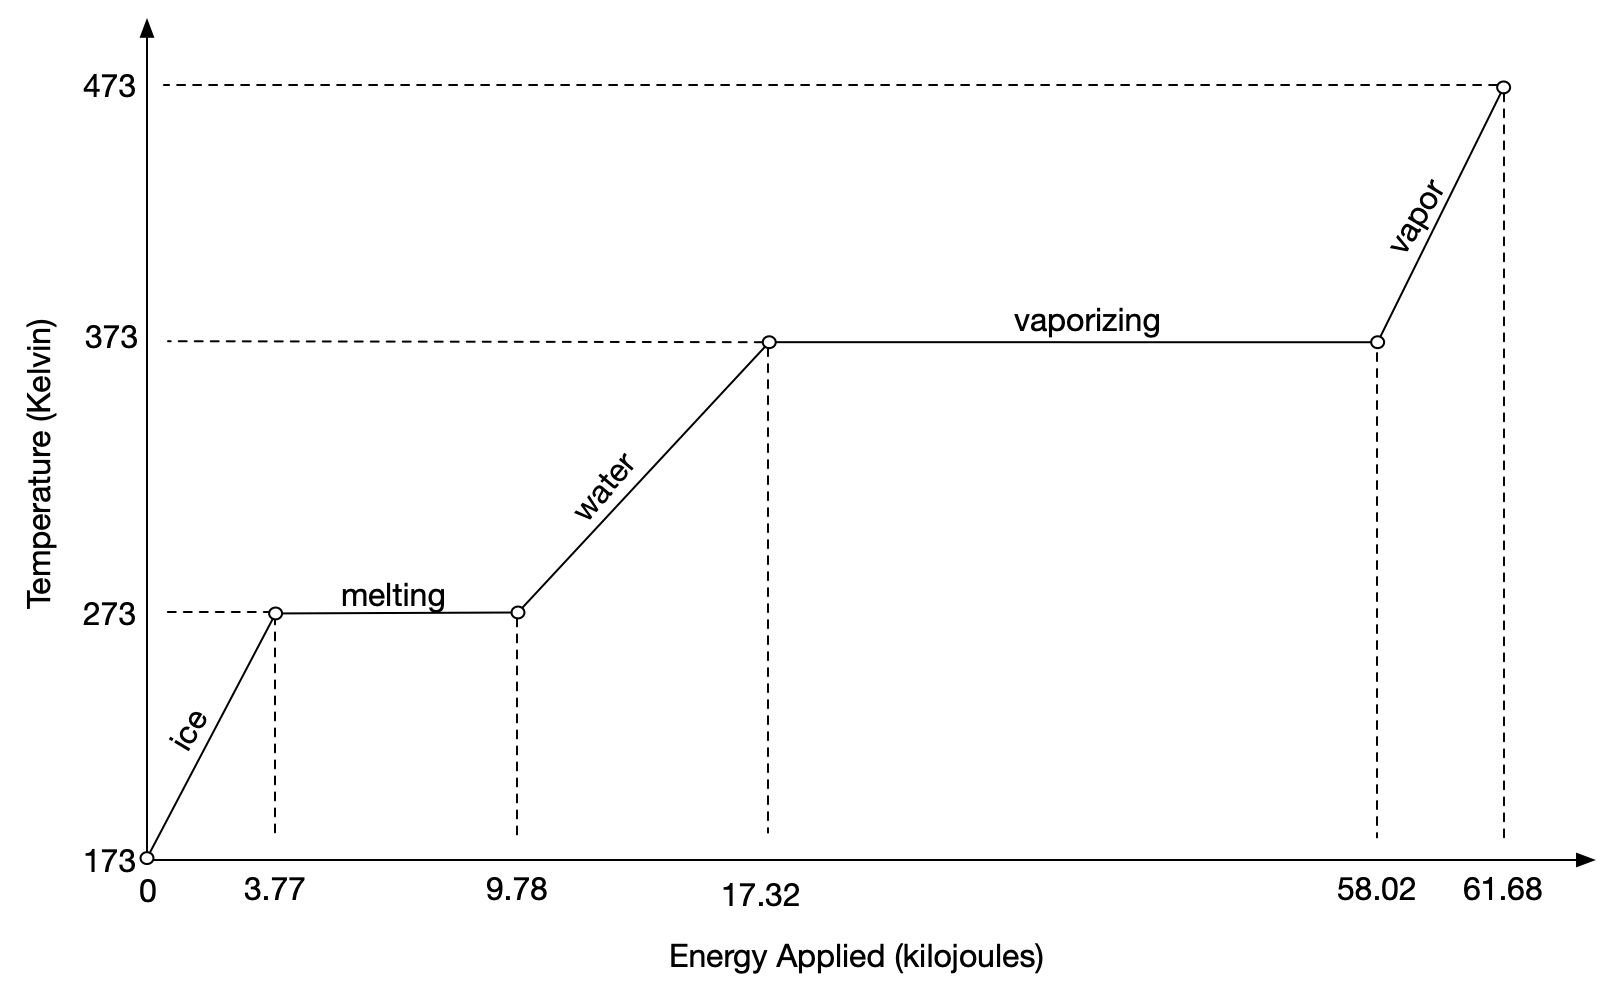
\includegraphics[width=0.8\linewidth]{energysoph.png}
    \caption{Actual temperature vs. energy applied.}
    \label{fig:energy2}
\end{figure}

Note that just as melting and vaporizing require energy, going the other way (freezing and condensing, respectively) give off energy. Thus, we can store energy using the phase change.

\subsection{How a Rice Cooker Works}\index{rice cooker}

A rice cooker is a bowl with a lid and an electric heating element. You put rice and water into the bowl and turn on the heating element. The heating element pushes kinetic energy into the water, which gets warmer and eventually starts to boil.

How does the rice cooker know when to turn off (or at least down to a low-heat "keep warm" mode) before the rice starts to burn?

As long as there is a little liquid water in the bottom of the bowl, the rice will not burn, so the question is really "How does it know when there is no more liquid water in the bottom of the bowl?"

There is a mechanism (and there have been a few different versions of this mechanism) that monitors the temperature of the surface of the bowl. As long as there is liquid water in the bowl, it \emph{cannot} go above $100^\circ$ C! When all the water has been absorbed by the rice or turned to steam, the temperature rises above $100^\circ$ C, and the mechanism cuts off the heat.
\begin{figure}[H]
    \centering
    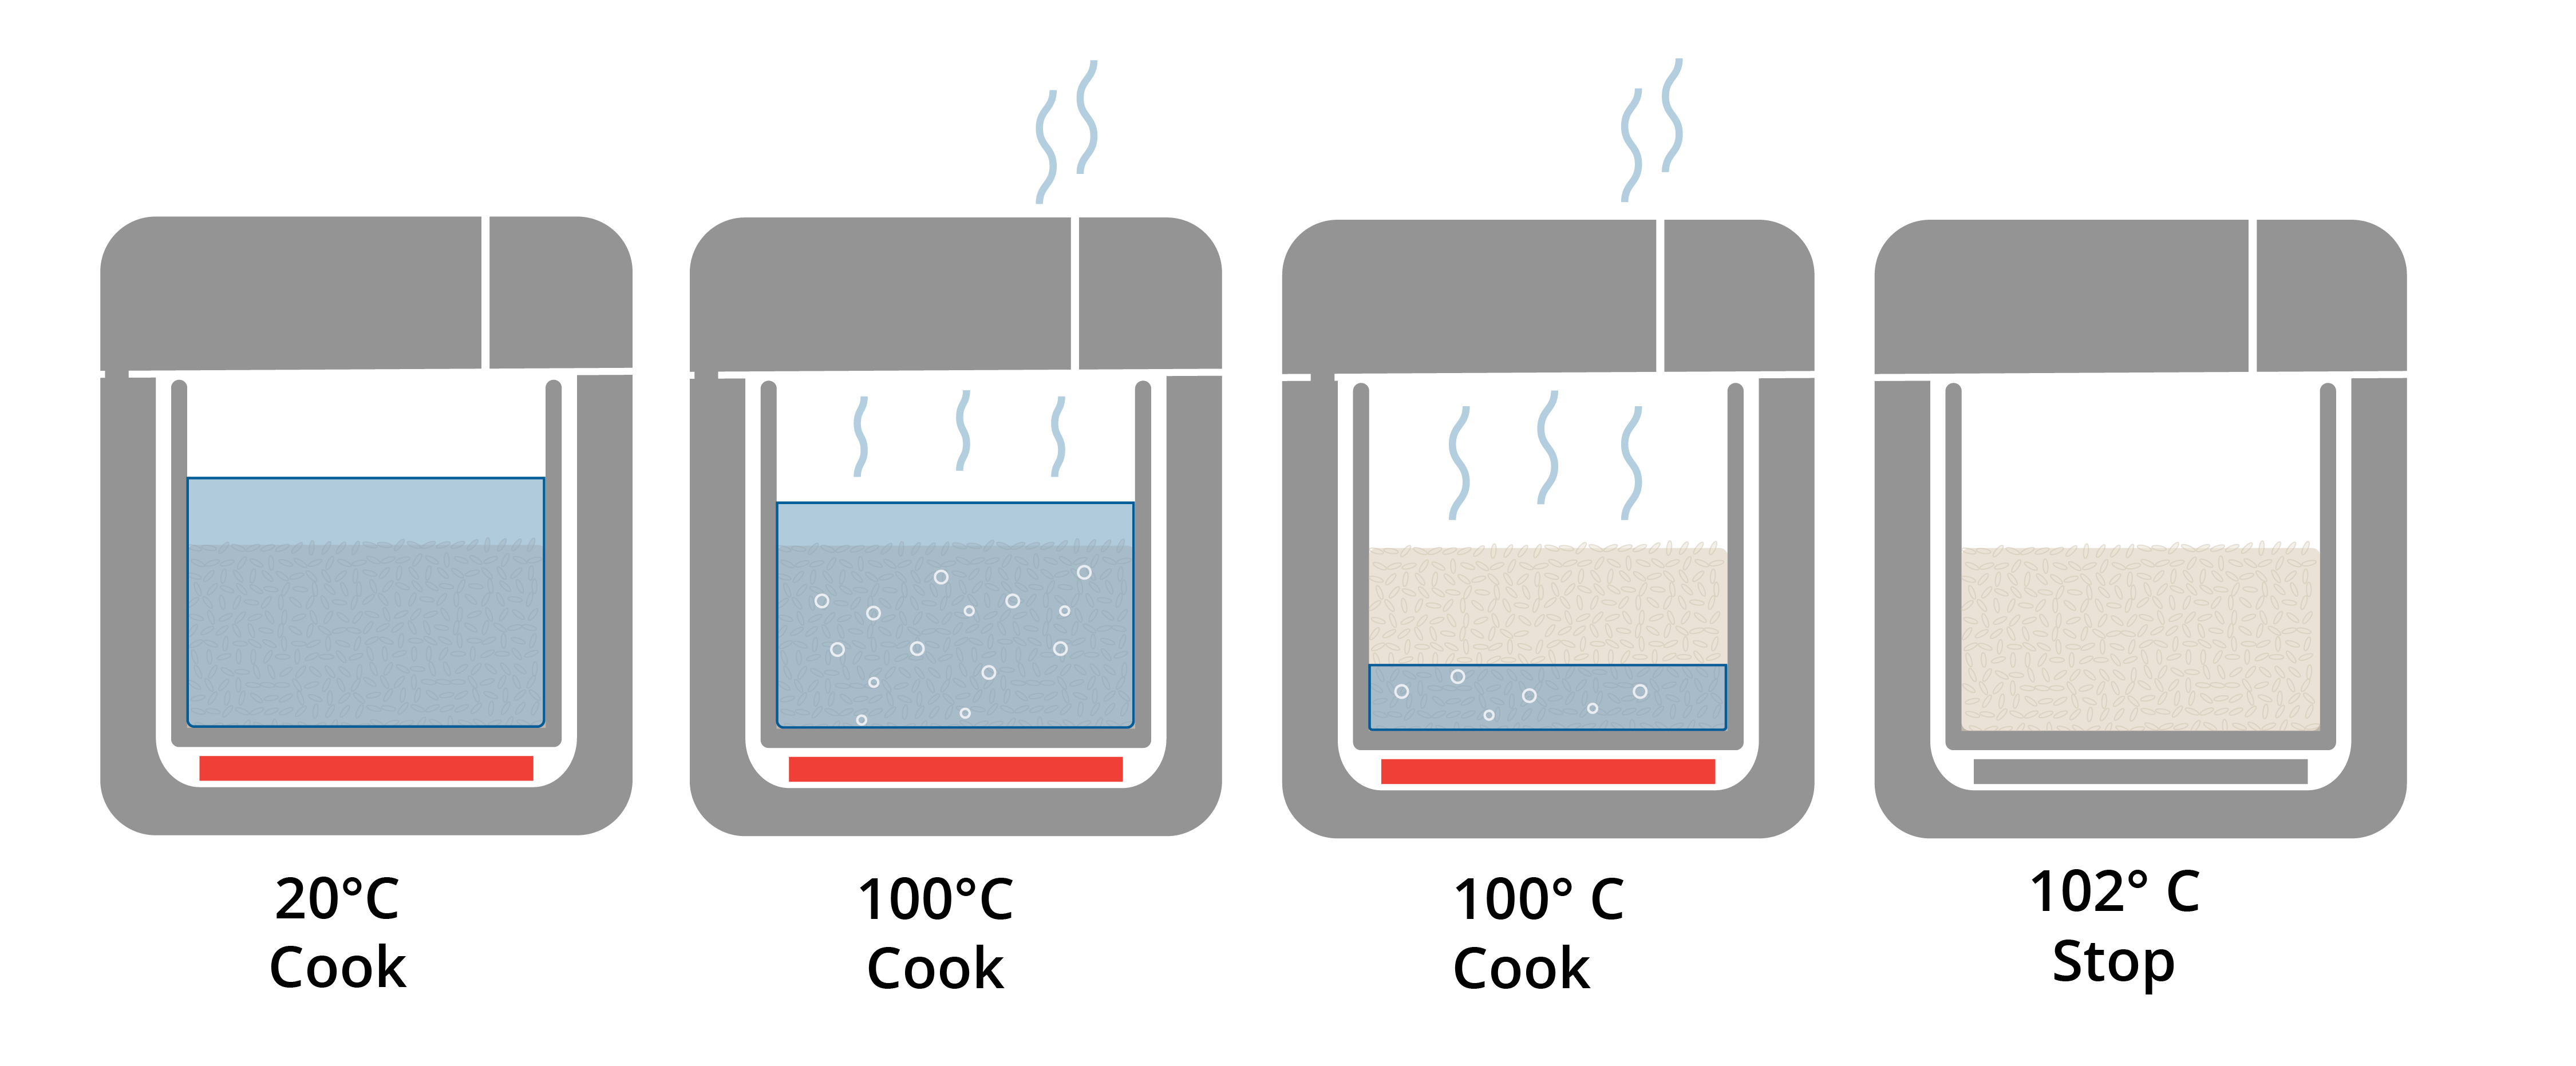
\includegraphics[width=0.9\linewidth]{riceCookerPhase.png}
    \caption{The various phases of a rice cooker.}
    \label{fig:riceCookerPhase}
\end{figure}

%FIXME could be good to add how does a pressure cooker work? if it adds any extra insight

\begin{Exercise}[title={Using Water For Thermal Energy Storage}, label=waterthermal]
Tom is building a passive solar house; the front of the house is a greenhouse, and Tom likes to 
eat dinner there. Tom plans to use barrels (painted black) that hold 159 liters of water. The plan is to let the sun heat the barrels to $33^\circ$ C by the time the sun goes down. (Any warmer and it would be unpleasant to eat dinner near them.)

At night, air will circulate past the barrels and through the house. Tom is OK with the house and the barrels dropping to $17^\circ$ C.

Looking at the house's insulation and the expected nighttime temperatures, Tom estimates that the barrels need to store 300,000 kJ of energy in the barrels.

A mole of water is about 0.018 liters.

The molar heat capacity of water is about 75.38 J/mole-K.

How many barrels of water does Tom need to install in the greenhouse?

\end{Exercise}
\begin{Answer}[ref=waterthermal] 

When one mole of water goes from $33^\circ$ to $17^\circ$, it will give off $(75.38)(33-17) = 1,206$ Joules or $1.206$ kJ. 

Tom needs 300,000 kJ, which takes $300,000/1.206 =  248,739.72$ moles of water.

How many liters is that? $248,739.72 * 0.018 = 4,477.31$ liters.

How many barrels is that? $4,477.31 / 159 = 28.16$ barrels. Tom will need 29 barrels.
 
\end{Answer}


\begin{Exercise}[title={Using Mirabilite For Thermal Energy Storage}, label=mirabilite]

Water barrels are going to take up too much of Tom's greenhouse!

There is a substance known as mirabilite, or Glauber's salt, or sodium sulfate decahydrate. It is relatively cheap to produce, and it has a melting point of $32.4^\circ$ C.

The molar heat capacity of mirabilite is 550 J/mole-K.

The latent heat of melting mirabilite is 82 kJ per mole.

Mirabilite comes in a powder form. Assume that a mole of mirabilite occupies about 0.22 liters.

If Tom fills the barrels with mirabilite instead, how many barrels are needed?

\end{Exercise}
\begin{Answer}[ref=mirabilite] 

When one mole of mirabilite goes from $33^\circ$ to $17^\circ$, it will give off $(550)(33-17) + 82,000 = 90,800$ Joules or $90.8$ kJ. 

Tom needs 300,000 kJ, which takes $300,000/90.8 =  3,304$ moles of mirabilite.

How many liters is that? $3,304 * 0.22 = 726.9$ liters.

How many barrels is that? $726.9 / 159 = 4.57$. Tom will need 5 barrels.
 
\end{Answer}

\subsection{Thinking Statistically About Phase Change}\index{evaporation}

We like to say simple things like "At $100^\circ$ C, water changes to vapor." However, remember what
temperature is: Temperature tells you how much average kinetic energy the water molecules have.  The key word here is \emph{average}; Some molecules are going faster than average and some are going slower.

A puddle in the street on a warm night will evaporate. It is not $100^\circ$ C. Why would the puddle turn to vapor?

While the \emph{average} molecule in the puddle does not have enough energy to escape the intermolecular forces, some of the molecules do. When a molecule on the surface has enough velocity (toward the sky!) to escape the intermolecular forces, it becomes vapor and leaves the puddle.

What happens to the temperature of the puddle during this sort of evaporation? Temperature is proportional to the average kinetic energy of the molecules. If a bunch of molecules with a lot of kinetic energy leave, the average kinetic energy (of the molecules that remain) will decrease.

The most obvious example of this process is sweating: When your body is in danger of getting too hot, sweat comes out of your pores and covers your body. The fastest moving molecules escape your body, taking the excess kinetic energy with them.

\subsubsection{Evaporative Cooling Systems}\index{evaporative cooling}

An evaporative cooling system (also called a "Swamp Cooler") uses this idea to cool air. You can imagine a fan drawing warm air through a duct from the outside.  Before the air is released inside, it passes very close to a cloth that is soaked with water.  The warm air molecules (which have a lot of kinetic energy) slam into the water molecules, some of which get enough kinetic energy to become vapor. The cool air and the water vapor then enter the room.

"Wait, wait, wait," you say, "The heat has not gone away. It is just transferred into the water molecules."

Remember that it takes 40.7 kilojoules to change a mole of liquid water at $100^\circ$ C to water vapor at $100^\circ$. Escaping those intermolecular bonds takes a great deal of energy!

Thus, if a mole of water evaporates, it has absorbed 40.7 kJ of heat that does not raise its temperature. The energy goes into breaking the molecules free of their intermolecular bonds. Physicists call this \newterm{latent heat}.
 
 \subsection{Humidity and Condensation}
 
When a puddle is evaporating on a warm day, there might be some water vapor already in the air. Even as the water molecules in the puddle are evaporating, some water molecules in the air are crashing into the puddle and become liquid again. (We say they \newterm{condensed}, thus the word \newterm{condensation} to describe the water that accumulates on a cold glass on a warm day.)
 
When there is a lot of water vapor in the air, the puddle will evaporate more slowly.  In fact, if there is enough
water vapor in the air, the puddle will not evaporate at all.  At this point, we say "The relative humidity is 100\%."  That is, relative to the amount of water the air will hold, it already has 100\% that amount.

Neither sweating nor evaporative cooling systems work well when the relative humidity is high.

As the temperature goes up, the air can hold more water. We usually notice it when it goes the other way: the air cools and has more water vapor than it can hold. Some of the water vapor condenses into water droplets. If the droplets land on something, we call it "dew". If it is high in the sky, we call the droplets "a cloud". If it is near the ground, we call it "fog".



 
